\section{plugin Class Reference}
\label{classplugin}\index{plugin@{plugin}}
The plugin base class.  


Inheritance diagram for plugin::\begin{figure}[H]
\begin{center}
\leavevmode
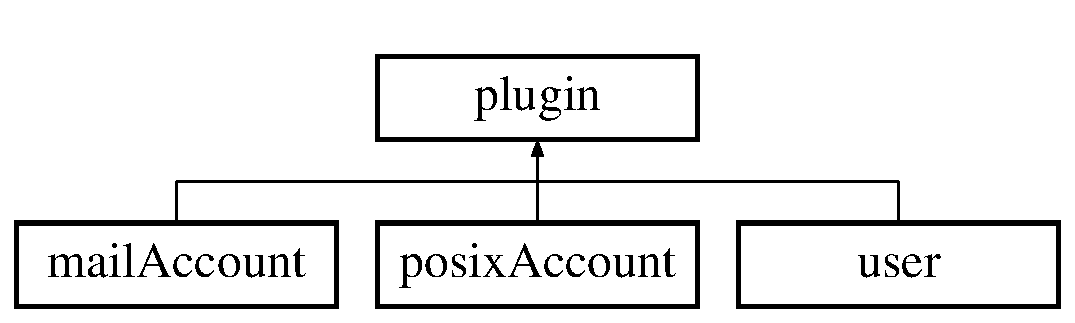
\includegraphics[height=2cm]{classplugin}
\end{center}
\end{figure}
\subsection*{Public Member Functions}
\begin{CompactItemize}
\item 
{\bf plugin} (\${\bf dn}=NULL)
\begin{CompactList}\small\item\em plugin constructor \item\end{CompactList}\item 
{\bf execute} ()
\begin{CompactList}\small\item\em execute plugin \item\end{CompactList}\item 
{\bf remove\_\-from\_\-parent} ()\label{classplugin_a2}

\item 
{\bf save\_\-object} ()\label{classplugin_a3}

\item 
{\bf save} ()\label{classplugin_a4}

\item 
{\bf check} ()\label{classplugin_a5}

\item 
{\bf adapt\_\-from\_\-template} (\${\bf dn})\label{classplugin_a6}

\item 
{\bf password\_\-change\_\-needed} ()\label{classplugin_a7}

\end{CompactItemize}
\subsection*{Public Attributes}
\begin{CompactItemize}
\item 
{\bf parent} = NULL
\begin{CompactList}\small\item\em Reference to parent object. \item\end{CompactList}\item 
{\bf is\_\-account} = FALSE
\begin{CompactList}\small\item\em Mark plugin as account. \item\end{CompactList}\item 
{\bf is\_\-template} = FALSE
\begin{CompactList}\small\item\em Mark plugin as template. \item\end{CompactList}\item 
{\bf attrs} = array()
\begin{CompactList}\small\item\em Represent temporary LDAP data. \item\end{CompactList}\item 
{\bf dn} = \char`\"{}\char`\"{}
\begin{CompactList}\small\item\em Used standard values. \item\end{CompactList}\item 
{\bf uid} = \char`\"{}\char`\"{}\label{classplugin_o5}

\item 
{\bf sn} = \char`\"{}\char`\"{}\label{classplugin_o6}

\item 
{\bf given\-Name} = \char`\"{}\char`\"{}\label{classplugin_o7}

\item 
{\bf acl} = \char`\"{}$\ast$none$\ast$\char`\"{}\label{classplugin_o8}

\item 
{\bf attributes} = array()\label{classplugin_o9}

\item 
{\bf objectclasses} = array()\label{classplugin_o10}

\end{CompactItemize}


\subsection{Detailed Description}
The plugin base class. 

\begin{Desc}
\item[Author:]Cajus Pollmeier $<${\tt pollmeier@gonicus.de}$>$ \end{Desc}
\begin{Desc}
\item[Version:]2.00 \end{Desc}
\begin{Desc}
\item[Date:]24.07.2003\end{Desc}
This is the base class for all plugins. It can be used standalone or can be included by the tabs class. All management should be done within this class. Extend your plugins from this class. 



\subsection{Constructor \& Destructor Documentation}
\index{plugin@{plugin}!plugin@{plugin}}
\index{plugin@{plugin}!plugin@{plugin}}
\subsubsection{\setlength{\rightskip}{0pt plus 5cm}plugin::plugin (\$ {\em dn} = NULL)}\label{classplugin_a0}


plugin constructor 

If 'dn' is set, the node loads the given 'dn' from LDAP

\begin{Desc}
\item[Parameters:]
\begin{description}
\item[{\em dn}]Distinguished name to initialize plugin from \end{description}
\end{Desc}
\begin{Desc}
\item[See also:]{\bf plugin()} \end{Desc}


\subsection{Member Function Documentation}
\index{plugin@{plugin}!execute@{execute}}
\index{execute@{execute}!plugin@{plugin}}
\subsubsection{\setlength{\rightskip}{0pt plus 5cm}plugin::execute ()}\label{classplugin_a1}


execute plugin 

Generates the html output for this node 

Reimplemented in {\bf mail\-Account} {\rm (p.\,\pageref{classmailAccount_a4})}, {\bf posix\-Account} {\rm (p.\,\pageref{classposixAccount_a1})}, and {\bf user} {\rm (p.\,\pageref{classuser_a1})}.

\subsection{Member Data Documentation}
\index{plugin@{plugin}!attrs@{attrs}}
\index{attrs@{attrs}!plugin@{plugin}}
\subsubsection{\setlength{\rightskip}{0pt plus 5cm}{\bf plugin::attrs} = array()}\label{classplugin_o3}


Represent temporary LDAP data. 

This is only used internally. \index{plugin@{plugin}!dn@{dn}}
\index{dn@{dn}!plugin@{plugin}}
\subsubsection{\setlength{\rightskip}{0pt plus 5cm}{\bf plugin::dn} = \char`\"{}\char`\"{}}\label{classplugin_o4}


Used standard values. 

dn \index{plugin@{plugin}!is_account@{is\_\-account}}
\index{is_account@{is\_\-account}!plugin@{plugin}}
\subsubsection{\setlength{\rightskip}{0pt plus 5cm}{\bf plugin::is\_\-account} = FALSE}\label{classplugin_o1}


Mark plugin as account. 

Defines whether this plugin is defined as an account or not. This has consequences for the plugin to be saved from tab mode. If it is set to 'FALSE' the tab will call the delete function, else the save function. Should be set to 'TRUE' if the construtor detects a valid LDAP object.

\begin{Desc}
\item[See also:]{\bf plugin::plugin()} \end{Desc}
\index{plugin@{plugin}!is_template@{is\_\-template}}
\index{is_template@{is\_\-template}!plugin@{plugin}}
\subsubsection{\setlength{\rightskip}{0pt plus 5cm}{\bf plugin::is\_\-template} = FALSE}\label{classplugin_o2}


Mark plugin as template. 

Defines whether we are creating a template or a normal object. Has conseqences on the way {\bf execute()} shows the formular and how save() puts the data to LDAP.

\begin{Desc}
\item[See also:]plugin::save() {\bf plugin::execute()} \end{Desc}
\index{plugin@{plugin}!parent@{parent}}
\index{parent@{parent}!plugin@{plugin}}
\subsubsection{\setlength{\rightskip}{0pt plus 5cm}{\bf plugin::parent} = NULL}\label{classplugin_o0}


Reference to parent object. 

This variable is used when the plugin is included in tabs and keeps reference to the tab class. Communication to other tabs is possible by 'name'. So the 'fax' plugin can ask the 'userinfo' plugin for the fax number.

\begin{Desc}
\item[See also:]tab \end{Desc}


The documentation for this class was generated from the following file:\begin{CompactItemize}
\item 
plugin.inc\end{CompactItemize}
